%%%--------------------------------%%%
%%% UC1
%%%--------------------------------%%%

\newpage
% UC1 ====================================================
\subsubsection{Use Case Specification: \ac{UC}1 User CRUD}
\label{sec:domainBbb}

\paragraph*{Description}\mbox{}\\
This use case specifies how user accounts are being created, updated, deleted and are used for login and logout.
These fields are required for the user account creation:

\begin{itemize}
	\vspace{-3mm}
	\setlength\itemsep{-1em}
	\item e-mail adress (String)
	\item password (String)
\end{itemize}
Additionaly the user can set the following field while updating his account:
\begin{itemize}
	\vspace{-3mm}
	\setlength\itemsep{-1em}
	\item language (enum)
\end{itemize}

\paragraph*{Screenshots}\mbox{}\\
Insert screenshots and shortly explain what can be seen
\begin{figure}[h] 
	\centering
	
\includegraphics[width=0.1\textwidth]{Content/Domain/placeholder.png}
	\caption{Use Case X: Detail}
	\label{fig:useCaseXDetailY}
\end{figure}

\newpage
\paragraph*{Basic Flow} \mbox{}\\
\noindent
New Account:
\begin{itemize}
	\vspace{-3mm}
	\setlength\itemsep{-1em}
	
	\item The visitor clicks the "register" button and fills in the fields mentioned in the brief description.
	\item Then clicks on the "register" button below the form to send the input to the server.
	\item If the visitors input fulfills the criteria of a username, email and password the account is being created on the server and a conformation e-mail is send to the given e-mail address.
\end{itemize}
The account itself can only be used after by clicking on the provided link in the conformation e-mail.

\noindent
Update Account: 
\begin{itemize}
	\vspace{-3mm}
	\setlength\itemsep{-1em}
	\item The user is logged in and clicks on the "settings" button.
	\item After updating the the fields the user wants to change, the input is sent to the server.
	\item If the updated fields fulfill their criteria, those fields are updated on the server.
\end{itemize} 

\noindent
Delete Account:
\begin{itemize}
	\vspace{-3mm}
	\setlength\itemsep{-1em}
	\item The user is logged in and clicks on the "settings" button.
	\item The user then clicks on the "delete my profile" button. 
	\item After typing in the users password, the request to delete the profile can be send to the server by clicking on the "delete" button.
	\item If the given password match the user's password the account is being deleted on the server and user will be logged out.
\end{itemize}

\noindent
Login:
\begin{itemize}
	\vspace{-3mm}
	\setlength\itemsep{-1em}
	\item The visitor already created an account and wants to log in.
	\item Therefor the "login" button must be clicked and the e-mail and password fields have to be filled in.
	\item The visitor can then click the "login" button below the form.
	\item If the e-mail and password match an entry of the list of registered users, the visitor will be logged in and can act as an user.
\end{itemize}

\noindent
Logout:
\begin{itemize}
	\vspace{-3mm}
	\setlength\itemsep{-1em}
	\item The user is logged in and wants to log out.
	\item By clicking the "logout" button the client removes all information used to authenticate to the server and forces the user interface to render without any user specific information fetched from the server.
\end{itemize}
The user is now able to login again.


\newpage
\subparagraph{Activity Diagram}\mbox{}\\
\begin{figure}[H]
	\centering
	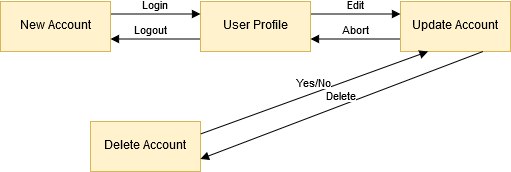
\includegraphics[width=0.9\textwidth]{Content/Domain/UC1UserCRUDactivitydiagram.png}
	\caption{Activity Diagram \ac{UC}1 User CRUD}
	\label{fig:activityDiagramUC1}
\end{figure}

\paragraph*{Alternative Flows}\mbox{}\\

\noindent
Invalid input: 
\begin{itemize}
	\vspace{-3mm}
	\setlength\itemsep{-1em}
	\item The user / visitor fills in the required fields (username, e-mail, password, language).
	\item If one field does not meet its criteria (e.g. an e-mail should contain the @-sign), which is validated by the server after submitting the input, the user / visitor will be informed next to the input fields.
\end{itemize} 
In this case the user account won't be created nor updated.

\noindent
Invalid user credentials:
\begin{itemize}
	\vspace{-3mm}
	\setlength\itemsep{-1em}
	\item If a visitor wants to login into an existing user account or if an account should be deleted by a user, the user accounts credentials have to be submitted (e-mail and password for login, password only for deletion).
	\item If the account credentials do not match any entry on the server, the user / visitor will be informed next to the input fields.
\end{itemize}
In this flow the visitor won't be logged in and neither will the account be deleted.

\paragraph*{Special Requirements and Preconditions}\mbox{}\\
Different flows require different preconditions.
\begin{enumerate}
	\vspace{-3mm}
	\setlength\itemsep{-1em}
	\item If a visitor wants to log into an user account has to exist or created beforehand.
	\item If a user wants to log out, the user has to be logged in.
	\item If a user wants to update or delete the account,the user has to be logged in, too.
\end{enumerate}

\paragraph*{Postconditions and Persistance}\mbox{}\\
Mentionable postconditions are:
\begin{enumerate}
	\vspace{-3mm}
	\setlength\itemsep{-1em}
	\item After deleting an account, the account can not be restored and therefor not being used anymore.
	\item Furthermore logging in allows a user to then access user related content from the server and logging out hides all user related content respectively.
\end{enumerate}

\noindent
The persistence guidelines are: 
\newline
\noindent
Creating, updating and deleting a user account or logging in by filling in the required fields and then submitting the input leads to a POST request to the server. If the fields fulfill their criteria, the information will be persisted on the server. Logging out will only delete the users authentication information on the client side and will not send a request to the server.

